\documentclass[tikz,border=6pt]{standalone}
% ============================================================================
%  VeriGate diagram design system (shared by every standalone figure).
%  Goals: bold, legible, print-safe; shape carries notation, colour reinforces
%  outcome; arrow labels sit on tinted pills so they never erase the arrow line;
%  no mid-word hyphenation inside nodes.
% ============================================================================
\usepackage[T1]{fontenc}
\usepackage{fouriernc}
\usetikzlibrary{arrows.meta,positioning,calc,fit,shapes.geometric,shapes.symbols,shapes.misc,backgrounds,shadows.blur}

% --- Never hyphenate words inside nodes (the main "sloppy / AI" tell) ---
\hyphenpenalty=10000
\exhyphenpenalty=10000
\tolerance=2000
\hbadness=10000

% --- Palette: cohesive, saturated enough to read, safe in grayscale ---
\definecolor{vgNavy}{HTML}{1F4E79}   % processes / primary
\definecolor{vgTeal}{HTML}{0E7C86}   % success / interaction
\definecolor{vgAmber}{HTML}{C8841B}  % decisions
\definecolor{vgSlate}{HTML}{4C5A68}  % external entities / stores
\definecolor{vgRed}{HTML}{C0453B}    % errors / reject / deny
\definecolor{vgGreen}{HTML}{2E8B57}  % final success outcome
\definecolor{vgViolet}{HTML}{6A4C93} % highlight / novel step
\definecolor{vgInk}{HTML}{2A3440}    % arrows & strokes
\definecolor{vgPaper}{HTML}{F4F1EA}  % label-pill background

\tikzset{
  % ---------- shared helpers ----------
  vgshadow/.style={blur shadow={shadow blur steps=5,shadow xshift=0.5pt,
      shadow yshift=-0.7pt,shadow opacity=28,shadow blur radius=1.4pt}},
  >={Stealth[length=2.6mm,width=2.1mm]},
  % ---------- data-flow (Yourdon/DeMarco) ----------
  dfdprocess/.style={circle,draw=vgNavy,line width=1.1pt,fill=vgNavy!14,
    align=center,font=\large\bfseries,text width=2.55cm,minimum size=3.15cm,
    inner sep=2pt,vgshadow},
  dfdentity/.style={rectangle,rounded corners=2pt,draw=vgSlate,line width=1pt,
    fill=vgSlate!14,align=center,font=\large,text width=2.6cm,minimum height=1.25cm,
    inner sep=5pt,vgshadow},
  dfdstore/.style={draw=none,align=center,font=\large,text width=3.1cm,
    minimum height=1.05cm,inner sep=4pt,
    append after command={\pgfextra{%
      \fill[vgTeal!8] (\tikzlastnode.north west) rectangle (\tikzlastnode.south east);
      \draw[vgSlate,line width=1pt]
        (\tikzlastnode.north west)--(\tikzlastnode.north east)
        (\tikzlastnode.south west)--(\tikzlastnode.south east);
      \draw[vgSlate,line width=1pt]
        ([xshift=5mm]\tikzlastnode.north west)--([xshift=5mm]\tikzlastnode.south west);}}},
  dfdflow/.style={-{Stealth[length=2.6mm,width=2.1mm]},line width=1pt,draw=vgInk,
    rounded corners=2pt},
  dfdlabel/.style={font=\normalsize,align=center,fill=vgPaper,draw=vgSlate!45,
    line width=0.3pt,rounded corners=2pt,inner sep=2.6pt},
  % ---------- flowcharts ----------
  fcstart/.style={rounded rectangle,draw=vgTeal,line width=1.1pt,fill=vgTeal!16,
    align=center,font=\normalsize\bfseries,text=vgInk,minimum height=10mm,
    inner sep=5pt,vgshadow},
  fcgo/.style={fcstart,draw=vgGreen,fill=vgGreen!16},           % final success
  fcerror/.style={fcstart,draw=vgRed,fill=vgRed!14},            % error / deny exit
  fcstep/.style={rectangle,rounded corners=3.5pt,draw=vgNavy,line width=1pt,
    fill=vgNavy!12,align=center,font=\normalsize,text=vgInk,text width=3.6cm,
    minimum height=11mm,inner sep=5pt,vgshadow},
  fckey/.style={fcstep,draw=vgViolet,line width=1.3pt,fill=vgViolet!14,
    font=\normalsize\bfseries},                                 % highlighted step
  fcdecision/.style={diamond,aspect=2.1,draw=vgAmber,line width=1.1pt,
    fill=vgAmber!22,align=center,font=\normalsize\bfseries,text=vgInk,
    text width=2.7cm,inner sep=1pt,vgshadow},
  fcarrow/.style={-{Stealth[length=2.6mm,width=2.1mm]},line width=1pt,draw=vgInk,
    rounded corners=3pt},
  fclabel/.style={font=\small\bfseries,fill=vgPaper,draw=vgSlate!45,line width=0.3pt,
    rounded corners=2pt,inner sep=2.4pt,align=center},
  fcyes/.style={fclabel,text=vgGreen,draw=vgGreen!50},
  fcno/.style={fclabel,text=vgRed,draw=vgRed!50},
  % ---------- sequence (kept for compatibility) ----------
  sqhead/.style={rectangle,rounded corners=2pt,draw=vgNavy,line width=1pt,
    fill=vgNavy!14,align=center,font=\normalsize\bfseries,minimum height=9mm,
    text width=2.3cm,inner sep=2pt,vgshadow},
  sqlife/.style={densely dashed,draw=vgSlate!60,line width=.6pt},
  sqcall/.style={-{Stealth[length=2.6mm]},line width=1pt,draw=vgInk},
  sqreply/.style={-{Stealth[length=2.6mm]},dashed,line width=.8pt,draw=vgInk},
  sqlabel/.style={font=\small,fill=vgPaper,draw=vgSlate!45,line width=.3pt,
    rounded corners=2pt,inner sep=2.2pt},
  sqframe/.style={draw=vgSlate,line width=.8pt,fill=white},
  sqtag/.style={font=\small,anchor=north west,draw=vgSlate,fill=vgTeal!18,inner sep=2pt},
  % ---------- deployment / components ----------
  component/.style={rectangle,rounded corners=3pt,draw=vgNavy,line width=1pt,
    fill=vgNavy!12,align=center,font=\normalsize,text=vgInk,minimum height=11mm,
    inner sep=6pt,vgshadow},
  comphi/.style={component,draw=vgTeal,line width=1.2pt,fill=vgTeal!14},
  boundary/.style={rectangle,rounded corners=4pt,draw=vgSlate,line width=1pt,
    fill=vgSlate!6,inner sep=3pt},
  link/.style={-{Stealth[length=2.6mm,width=2.1mm]},line width=1pt,draw=vgInk,
    rounded corners=2pt},
  linklabel/.style={font=\small\bfseries,fill=vgPaper,draw=vgSlate!45,line width=.3pt,
    rounded corners=2pt,inner sep=2.4pt,align=center},
  statelabel/.style={rectangle,rounded corners=3pt,draw=vgNavy,line width=1pt,
    fill=vgNavy!14,align=center,font=\normalsize,minimum height=10mm,inner sep=5pt,vgshadow}
}

\definecolor{vgNavy}{HTML}{88421D}\definecolor{vgTeal}{HTML}{52B788}
\begin{document}
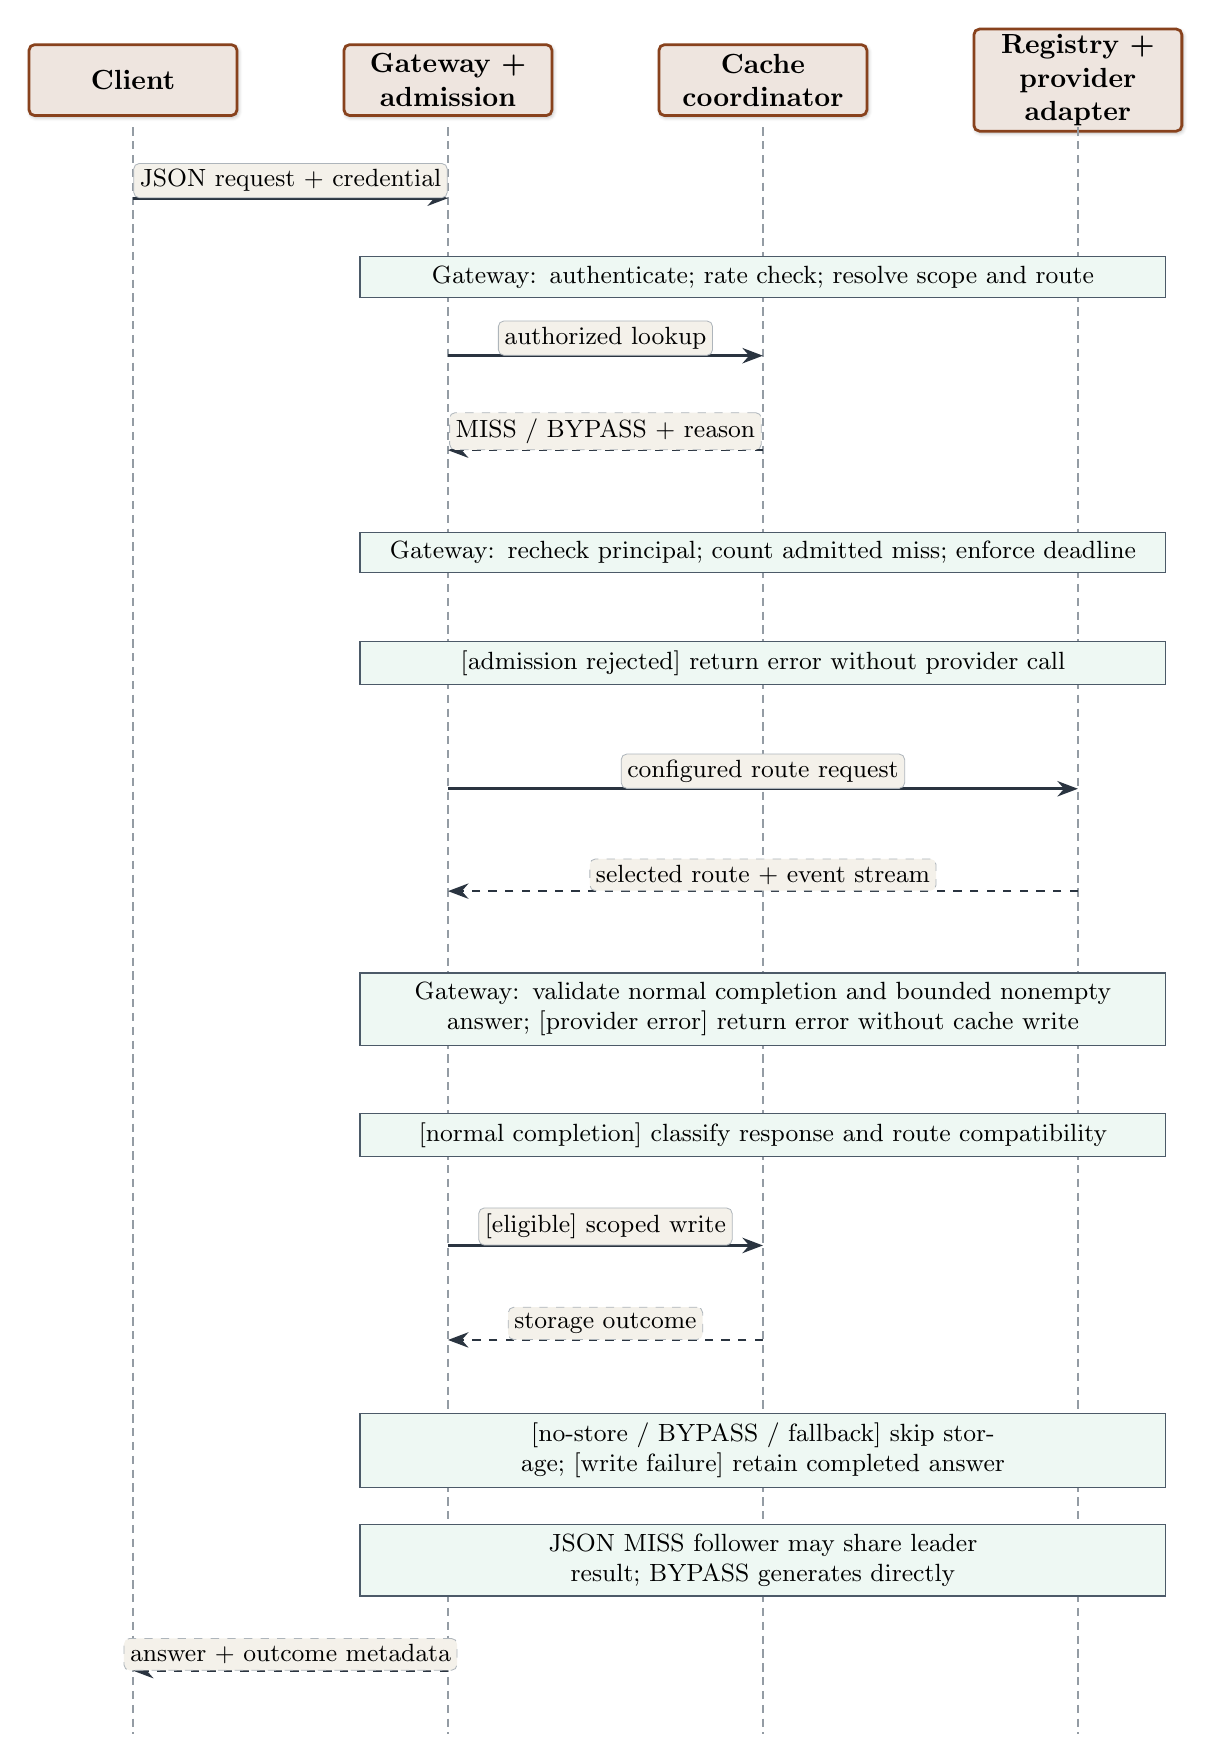
\begin{tikzpicture}
\tikzset{sqhead/.append style={text width=2.5cm},sqlabel/.append style={font=\small}}
\node[sqhead] at (0,0) {Client};\draw[sqlife] (0,-.6)--(0,-21);
\node[sqhead] at (4,0) {Gateway +\\admission};\draw[sqlife] (4,-.6)--(4,-21);
\node[sqhead] at (8,0) {Cache coordinator};\draw[sqlife] (8,-.6)--(8,-21);
\node[sqhead] at (12,0) {Registry +\\provider adapter};\draw[sqlife] (12,-.6)--(12,-21);
\draw[sqcall] (0,-1.5)--node[sqlabel,above,align=center]{JSON request + credential}(4,-1.5);
\draw[sqcall] (4,-3.5)--node[sqlabel,above,align=center]{authorized lookup}(8,-3.5);
\draw[sqreply] (8,-4.7)--node[sqlabel,above,align=center]{MISS / BYPASS + reason}(4,-4.7);
\draw[sqcall] (4,-9)--node[sqlabel,above,align=center]{configured route request}(12,-9);
\draw[sqreply] (12,-10.3)--node[sqlabel,above,align=center]{selected route + event stream}(4,-10.3);
\draw[sqcall] (4,-14.8)--node[sqlabel,above,align=center]{[eligible] scoped write}(8,-14.8);
\draw[sqreply] (8,-16)--node[sqlabel,above,align=center]{storage outcome}(4,-16);
\draw[sqreply] (4,-20.2)--node[sqlabel,above,align=center]{answer + outcome metadata}(0,-20.2);
\node[draw=vgSlate,fill=vgTeal!10,align=center,text width=10cm,font=\small] at (8,-2.5) {Gateway: authenticate; rate check; resolve scope and route};
\node[draw=vgSlate,fill=vgTeal!10,align=center,text width=10cm,font=\small] at (8,-6) {Gateway: recheck principal; count admitted miss; enforce deadline};
\node[draw=vgSlate,fill=vgTeal!10,align=center,text width=10cm,font=\small] at (8,-7.4) {[admission rejected] return error without provider call};
\node[draw=vgSlate,fill=vgTeal!10,align=center,text width=10cm,font=\small] at (8,-11.8) {Gateway: validate normal completion and bounded nonempty answer; [provider error] return error without cache write};
\node[draw=vgSlate,fill=vgTeal!10,align=center,text width=10cm,font=\small] at (8,-13.4) {[normal completion] classify response and route compatibility};
\node[draw=vgSlate,fill=vgTeal!10,align=center,text width=10cm,font=\small] at (8,-17.4) {[no-store / BYPASS / fallback] skip storage; [write failure] retain completed answer};
\node[draw=vgSlate,fill=vgTeal!10,align=center,text width=10cm,font=\small] at (8,-18.8) {JSON MISS follower may share leader result; BYPASS generates directly};

\end{tikzpicture}
\end{document}
